\documentclass{book}
\usepackage[a4paper,top=2.5cm,bottom=2.5cm,left=2.5cm,right=2.5cm]{geometry}
\usepackage{makeidx}
\usepackage{natbib}
\usepackage{graphicx}
\usepackage{multicol}
\usepackage{float}
\usepackage{listings}
\usepackage{color}
\usepackage{ifthen}
\usepackage[table]{xcolor}
\usepackage{textcomp}
\usepackage{alltt}
\usepackage{ifpdf}
\ifpdf
\usepackage[pdftex,
            pagebackref=true,
            colorlinks=true,
            linkcolor=blue,
            unicode
           ]{hyperref}
\else
\usepackage[ps2pdf,
            pagebackref=true,
            colorlinks=true,
            linkcolor=blue,
            unicode
           ]{hyperref}
\usepackage{pspicture}
\fi
\usepackage[utf8]{inputenc}
\usepackage{mathptmx}
\usepackage[scaled=.90]{helvet}
\usepackage{courier}
\usepackage{sectsty}
\usepackage[titles]{tocloft}
\usepackage{doxygen}
\lstset{language=C++,inputencoding=utf8,basicstyle=\footnotesize,breaklines=true,breakatwhitespace=true,tabsize=8,numbers=left }
\makeindex
\setcounter{tocdepth}{3}
\renewcommand{\footrulewidth}{0.4pt}
\renewcommand{\familydefault}{\sfdefault}
\hfuzz=15pt
\setlength{\emergencystretch}{15pt}
\hbadness=750
\tolerance=750
\begin{document}
\hypersetup{pageanchor=false,citecolor=blue}
\begin{titlepage}
\vspace*{7cm}
\begin{center}
{\Large My Project }\\
\vspace*{1cm}
{\large Generated by Doxygen 1.8.1.1}\\
\vspace*{0.5cm}
{\small Thu Jun 28 2012 15:50:40}\\
\end{center}
\end{titlepage}
\clearemptydoublepage
\pagenumbering{roman}
\tableofcontents
\clearemptydoublepage
\pagenumbering{arabic}
\hypersetup{pageanchor=true,citecolor=blue}
\chapter{Proyecto\-Evolutiva}
\label{md_README}
\hypertarget{md_README}{}
Proyecto evolutiva Feb-\/\-Jun 2012 
\chapter{Bug List}
\label{bug}
\hypertarget{bug}{}

\begin{DoxyRefList}
\item[\label{bug__bug000001}%
\hypertarget{bug__bug000001}{}%
page \hyperlink{index}{Descripción del proyecto.} ]No funciona con entradas con funciones desordenadas 
\end{DoxyRefList}
\chapter{Class Index}
\section{Class List}
Here are the classes, structs, unions and interfaces with brief descriptions\-:\begin{DoxyCompactList}
\item\contentsline{section}{\hyperlink{structFuncionAptitud_1_1compare}{Funcion\-Aptitud\-::compare} }{\pageref{structFuncionAptitud_1_1compare}}{}
\item\contentsline{section}{\hyperlink{classCromosoma}{Cromosoma} \\*Clase cromosoma }{\pageref{classCromosoma}}{}
\item\contentsline{section}{\hyperlink{classCruce}{Cruce} \\*Clase para el manejo del \hyperlink{classCruce}{Cruce} de los cromosomas }{\pageref{classCruce}}{}
\item\contentsline{section}{\hyperlink{classFuncionAptitud}{Funcion\-Aptitud} \\*Clase para el manejo de la función de Aptitud }{\pageref{classFuncionAptitud}}{}
\item\contentsline{section}{\hyperlink{classFuncionSeleccionCruce}{Funcion\-Seleccion\-Cruce} \\*Clase para seleccionar el Mating pool }{\pageref{classFuncionSeleccionCruce}}{}
\item\contentsline{section}{\hyperlink{classMutacion}{Mutacion} \\*Clase para implementar mutación }{\pageref{classMutacion}}{}
\item\contentsline{section}{\hyperlink{classSeleccion}{Seleccion} \\*Clase para el manejo de la función de Aptitud }{\pageref{classSeleccion}}{}
\item\contentsline{section}{\hyperlink{classTablaDeVerdad}{Tabla\-De\-Verdad} \\*Clase \hyperlink{classTablaDeVerdad}{Tabla\-De\-Verdad} }{\pageref{classTablaDeVerdad}}{}
\end{DoxyCompactList}

\chapter{Class Documentation}
\hypertarget{structFuncionAptitud_1_1compare}{\section{Funcion\-Aptitud\-:\-:compare Struct Reference}
\label{structFuncionAptitud_1_1compare}\index{Funcion\-Aptitud\-::compare@{Funcion\-Aptitud\-::compare}}
}


{\ttfamily \#include $<$funcionaptitud.\-h$>$}

\subsection*{Public Member Functions}
\begin{DoxyCompactItemize}
\item 
\hypertarget{structFuncionAptitud_1_1compare_ac7400ce0c2f1c80b038e35282ec2e379}{bool {\bfseries operator()} (\hyperlink{classCromosoma}{Cromosoma} a, \hyperlink{classCromosoma}{Cromosoma} b) const }\label{structFuncionAptitud_1_1compare_ac7400ce0c2f1c80b038e35282ec2e379}

\end{DoxyCompactItemize}


\subsection{Detailed Description}
Estructura para realizar la comparación de la función sort 

The documentation for this struct was generated from the following file\-:\begin{DoxyCompactItemize}
\item 
funcionaptitud.\-h\end{DoxyCompactItemize}

\hypertarget{classCromosoma}{\section{Referencia de la Clase Cromosoma}
\label{classCromosoma}\index{Cromosoma@{Cromosoma}}
}


Clase cromosoma.  




{\ttfamily \#include $<$Cromosoma.\-h$>$}

\subsection*{Métodos públicos}
\begin{DoxyCompactItemize}
\item 
\hyperlink{classCromosoma_a8fca0c1bd72c65aac6c2f26494e2c5f9}{Cromosoma} (int num\-Clausulas, int num\-Variables, bool maxi\-Terminos)
\begin{DoxyCompactList}\small\item\em Constructor. \end{DoxyCompactList}\item 
\hyperlink{classCromosoma_a39310d043c187768ba83a1a9c921e966}{$\sim$\-Cromosoma} ()
\begin{DoxyCompactList}\small\item\em Destructor. \end{DoxyCompactList}\item 
bool \hyperlink{classCromosoma_a59d6a42685e8b6e983b496d8051e4168}{get} (int x, int y)
\begin{DoxyCompactList}\small\item\em get \end{DoxyCompactList}\item 
vector$<$ bool $>$ \hyperlink{classCromosoma_a400e7970b9e2d9995cbc6b1f4335fd51}{get\-Clausula} (int x)
\begin{DoxyCompactList}\small\item\em get\-Clausula \end{DoxyCompactList}\item 
void \hyperlink{classCromosoma_aaf002d2f7f9438e74eeba52892868e83}{set} (int x, int y, bool z)
\begin{DoxyCompactList}\small\item\em set \end{DoxyCompactList}\item 
int \hyperlink{classCromosoma_a53e4a3cda8f7a0b2233f0219579f7cc3}{get\-Numero\-Clausulas} ()
\begin{DoxyCompactList}\small\item\em get\-Numero\-Clausulas \end{DoxyCompactList}\item 
int \hyperlink{classCromosoma_a825104a1dd2a7595d119907c84fd2fd1}{get\-Numero\-Variables} ()
\begin{DoxyCompactList}\small\item\em get\-Numero\-Variables \end{DoxyCompactList}\item 
bool \hyperlink{classCromosoma_a8a75eb52e417f9c050c32969b56984e7}{obtener\-Salida} (int posicion\-Decimal)
\begin{DoxyCompactList}\small\item\em obtener\-Salida \end{DoxyCompactList}\item 
double \hyperlink{classCromosoma_a280c8232e95aec0c8dd627cd579abec6}{get\-Aptitud} ()
\begin{DoxyCompactList}\small\item\em get\-Aptitud \end{DoxyCompactList}\item 
void \hyperlink{classCromosoma_a158f2fe672e3232ebf07a5724a15fc2e}{set\-Aptitud} (double value)
\begin{DoxyCompactList}\small\item\em set\-Aptitud \end{DoxyCompactList}\end{DoxyCompactItemize}


\subsection{Descripción detallada}
Clase cromosoma. 

\begin{DoxyVerb}Clase cromosoma
\end{DoxyVerb}


Define un cromosoma como una matriz, donde la fila representa una claúsula y la columna el estado de una variable y su negada \begin{DoxyAuthor}{Autor}
Carlos Andres Delgado 

Edgar Andres Moncada 

Luis Felipe Vargas 
\end{DoxyAuthor}
\begin{DoxyVersion}{Versión}
1.\-0 
\end{DoxyVersion}
\begin{DoxyDate}{Fecha}
2012 
\end{DoxyDate}
\begin{DoxyCopyright}{Copyright}
G\-N\-U Public License. $\ast$ 
\end{DoxyCopyright}


\subsection{Documentación del constructor y destructor}
\hypertarget{classCromosoma_a8fca0c1bd72c65aac6c2f26494e2c5f9}{\index{Cromosoma@{Cromosoma}!Cromosoma@{Cromosoma}}
\index{Cromosoma@{Cromosoma}!Cromosoma@{Cromosoma}}
\subsubsection[{Cromosoma}]{\setlength{\rightskip}{0pt plus 5cm}Cromosoma\-::\-Cromosoma (
\begin{DoxyParamCaption}
\item[{int}]{num\-Clausulas, }
\item[{int}]{num\-Variables, }
\item[{bool}]{maxi\-Terminos}
\end{DoxyParamCaption}
)}}\label{classCromosoma_a8fca0c1bd72c65aac6c2f26494e2c5f9}


Constructor. 

Constructor de la clase \hyperlink{classCromosoma}{Cromosoma} 
\begin{DoxyParams}{Parámetros}
{\em num\-Clausulas} & es un número entero que representa el número de claúsulas que tendrá el cromosoma \\
\hline
{\em num\-Variables} & es número entero que representa el número de variable y su negada que tendrá el cromosoma \\
\hline
\end{DoxyParams}
\hypertarget{classCromosoma_a39310d043c187768ba83a1a9c921e966}{\index{Cromosoma@{Cromosoma}!$\sim$\-Cromosoma@{$\sim$\-Cromosoma}}
\index{$\sim$\-Cromosoma@{$\sim$\-Cromosoma}!Cromosoma@{Cromosoma}}
\subsubsection[{$\sim$\-Cromosoma}]{\setlength{\rightskip}{0pt plus 5cm}Cromosoma\-::$\sim$\-Cromosoma (
\begin{DoxyParamCaption}
{}
\end{DoxyParamCaption}
)}}\label{classCromosoma_a39310d043c187768ba83a1a9c921e966}


Destructor. 

Destructor de la clase \hyperlink{classCromosoma}{Cromosoma} 

\subsection{Documentación de las funciones miembro}
\hypertarget{classCromosoma_a59d6a42685e8b6e983b496d8051e4168}{\index{Cromosoma@{Cromosoma}!get@{get}}
\index{get@{get}!Cromosoma@{Cromosoma}}
\subsubsection[{get}]{\setlength{\rightskip}{0pt plus 5cm}bool Cromosoma\-::get (
\begin{DoxyParamCaption}
\item[{int}]{x, }
\item[{int}]{y}
\end{DoxyParamCaption}
)}}\label{classCromosoma_a59d6a42685e8b6e983b496d8051e4168}


get 

Obtiene un elemento específico de una claúsula 
\begin{DoxyParams}{Parámetros}
{\em x} & es un número entero que indica la claúsula deseada \\
\hline
{\em y} & es número entero que indica la variable deseada (recordar que están duplicada) normal y negada \\
\hline
\end{DoxyParams}
\hypertarget{classCromosoma_a280c8232e95aec0c8dd627cd579abec6}{\index{Cromosoma@{Cromosoma}!get\-Aptitud@{get\-Aptitud}}
\index{get\-Aptitud@{get\-Aptitud}!Cromosoma@{Cromosoma}}
\subsubsection[{get\-Aptitud}]{\setlength{\rightskip}{0pt plus 5cm}double Cromosoma\-::get\-Aptitud (
\begin{DoxyParamCaption}
{}
\end{DoxyParamCaption}
)}}\label{classCromosoma_a280c8232e95aec0c8dd627cd579abec6}


get\-Aptitud 

Obtiene la aptitud que tiene el cromosoma \begin{DoxyReturn}{Devuelve}
double que representa el valor de la aptitud del cromosoma 
\end{DoxyReturn}
\hypertarget{classCromosoma_a400e7970b9e2d9995cbc6b1f4335fd51}{\index{Cromosoma@{Cromosoma}!get\-Clausula@{get\-Clausula}}
\index{get\-Clausula@{get\-Clausula}!Cromosoma@{Cromosoma}}
\subsubsection[{get\-Clausula}]{\setlength{\rightskip}{0pt plus 5cm}vector$<$ bool $>$ Cromosoma\-::get\-Clausula (
\begin{DoxyParamCaption}
\item[{int}]{x}
\end{DoxyParamCaption}
)}}\label{classCromosoma_a400e7970b9e2d9995cbc6b1f4335fd51}


get\-Clausula 

Obtiene una claúsula 
\begin{DoxyParams}{Parámetros}
{\em x} & es un número entero que indica la claúsula deseada \\
\hline
\end{DoxyParams}
\hypertarget{classCromosoma_a53e4a3cda8f7a0b2233f0219579f7cc3}{\index{Cromosoma@{Cromosoma}!get\-Numero\-Clausulas@{get\-Numero\-Clausulas}}
\index{get\-Numero\-Clausulas@{get\-Numero\-Clausulas}!Cromosoma@{Cromosoma}}
\subsubsection[{get\-Numero\-Clausulas}]{\setlength{\rightskip}{0pt plus 5cm}int Cromosoma\-::get\-Numero\-Clausulas (
\begin{DoxyParamCaption}
{}
\end{DoxyParamCaption}
)}}\label{classCromosoma_a53e4a3cda8f7a0b2233f0219579f7cc3}


get\-Numero\-Clausulas 

Retorna el número de claúsulas que tiene el cromosoma 

Gráfico de llamadas a esta función\-:
\nopagebreak
\begin{figure}[H]
\begin{center}
\leavevmode
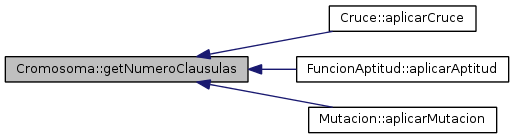
\includegraphics[width=350pt]{classCromosoma_a53e4a3cda8f7a0b2233f0219579f7cc3_icgraph}
\end{center}
\end{figure}


\hypertarget{classCromosoma_a825104a1dd2a7595d119907c84fd2fd1}{\index{Cromosoma@{Cromosoma}!get\-Numero\-Variables@{get\-Numero\-Variables}}
\index{get\-Numero\-Variables@{get\-Numero\-Variables}!Cromosoma@{Cromosoma}}
\subsubsection[{get\-Numero\-Variables}]{\setlength{\rightskip}{0pt plus 5cm}int Cromosoma\-::get\-Numero\-Variables (
\begin{DoxyParamCaption}
{}
\end{DoxyParamCaption}
)}}\label{classCromosoma_a825104a1dd2a7595d119907c84fd2fd1}


get\-Numero\-Variables 

Retorna el número de variables que tiene cada claúsula en el cromosoma \hypertarget{classCromosoma_a8a75eb52e417f9c050c32969b56984e7}{\index{Cromosoma@{Cromosoma}!obtener\-Salida@{obtener\-Salida}}
\index{obtener\-Salida@{obtener\-Salida}!Cromosoma@{Cromosoma}}
\subsubsection[{obtener\-Salida}]{\setlength{\rightskip}{0pt plus 5cm}bool Cromosoma\-::obtener\-Salida (
\begin{DoxyParamCaption}
\item[{int}]{posicion\-Decimal}
\end{DoxyParamCaption}
)}}\label{classCromosoma_a8a75eb52e417f9c050c32969b56984e7}


obtener\-Salida 

Obtiene una salida ante una entrada decimal de un cromosoma (En cualquier representación, maxitérminos o minitérminos) 
\begin{DoxyParams}{Parámetros}
{\em posicion\-Decimal} & es un número entero que representa la posición que se desea conocer \\
\hline
\end{DoxyParams}
\begin{DoxyReturn}{Devuelve}
booleano que representa el valor que toma la función ante la entrada especificada 
\end{DoxyReturn}


Gráfico de llamadas a esta función\-:
\nopagebreak
\begin{figure}[H]
\begin{center}
\leavevmode
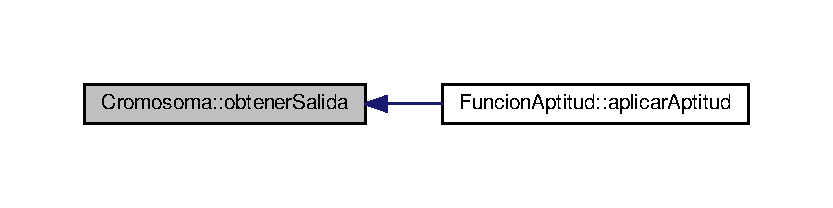
\includegraphics[width=350pt]{classCromosoma_a8a75eb52e417f9c050c32969b56984e7_icgraph}
\end{center}
\end{figure}


\hypertarget{classCromosoma_aaf002d2f7f9438e74eeba52892868e83}{\index{Cromosoma@{Cromosoma}!set@{set}}
\index{set@{set}!Cromosoma@{Cromosoma}}
\subsubsection[{set}]{\setlength{\rightskip}{0pt plus 5cm}void Cromosoma\-::set (
\begin{DoxyParamCaption}
\item[{int}]{x, }
\item[{int}]{y, }
\item[{bool}]{z}
\end{DoxyParamCaption}
)}}\label{classCromosoma_aaf002d2f7f9438e74eeba52892868e83}


set 

Obtiene un elemento específico de una claúsula 
\begin{DoxyParams}{Parámetros}
{\em x} & es un número entero que indica la claúsula deseada \\
\hline
{\em y} & es número entero que indica la variable deseada (recordar que están duplicada) normal y negada \\
\hline
{\em z} & es booleano que indica el valor de la variable y deseada en la claúsula x \\
\hline
\end{DoxyParams}
\hypertarget{classCromosoma_a158f2fe672e3232ebf07a5724a15fc2e}{\index{Cromosoma@{Cromosoma}!set\-Aptitud@{set\-Aptitud}}
\index{set\-Aptitud@{set\-Aptitud}!Cromosoma@{Cromosoma}}
\subsubsection[{set\-Aptitud}]{\setlength{\rightskip}{0pt plus 5cm}void Cromosoma\-::set\-Aptitud (
\begin{DoxyParamCaption}
\item[{double}]{value}
\end{DoxyParamCaption}
)}}\label{classCromosoma_a158f2fe672e3232ebf07a5724a15fc2e}


set\-Aptitud 

Establece la aptitud que tiene el cromosoma 

Gráfico de llamadas a esta función\-:
\nopagebreak
\begin{figure}[H]
\begin{center}
\leavevmode
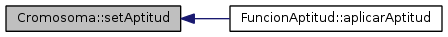
\includegraphics[width=350pt]{classCromosoma_a158f2fe672e3232ebf07a5724a15fc2e_icgraph}
\end{center}
\end{figure}




La documentación para esta clase fue generada a partir de los siguientes ficheros\-:\begin{DoxyCompactItemize}
\item 
Cromosoma.\-h\item 
Cromosoma.\-cpp\end{DoxyCompactItemize}

\hypertarget{classCruce}{\section{Referencia de la Clase Cruce}
\label{classCruce}\index{Cruce@{Cruce}}
}


Clase para el manejo del \hyperlink{classCruce}{Cruce} de los cromosomas.  




{\ttfamily \#include $<$cruce.\-h$>$}

\subsection*{Métodos públicos}
\begin{DoxyCompactItemize}
\item 
\hyperlink{classCruce_af0c3421f9764a791c63c08cd98a50b3b}{Cruce} (vector$<$ \hyperlink{classCromosoma}{Cromosoma} $\ast$ $>$ poblacion\-Seleccionada)
\begin{DoxyCompactList}\small\item\em Constructor. \end{DoxyCompactList}\item 
vector$<$ \hyperlink{classCromosoma}{Cromosoma} $\ast$ $>$ \hyperlink{classCruce_a5fd9d9cbca36abf7d81f5eedc06f18e7}{aplicar\-Cruce} ()
\begin{DoxyCompactList}\small\item\em Función que calculara los nuevos hijos al cruzar la población actual. \end{DoxyCompactList}\end{DoxyCompactItemize}


\subsection{Descripción detallada}
Clase para el manejo del \hyperlink{classCruce}{Cruce} de los cromosomas. 

\begin{DoxyVerb}Clase Cruce
\end{DoxyVerb}


Esta clase permitira realizar el cruce de los cromosomas. Se seleccionan dos cromosomas dentro del grupo de seleccionados, se toma el cromosoma con menor número de cláusulas y se genera un número aleatorio entre 1 y ese número menos 1, valor que se denota con alfa. Con éste valor se generan dos hijos, uno tomando en ambos cromosomas alfa claúsulas iniciales y generando un cromosoma de tamaño 2 ∗ alfa, con el resto de ambos cromosomas se realiza el mismo procedimiento. \begin{DoxyAuthor}{Autor}
Carlos Andres Delgado 

Edgar Andres Moncada 

Luis Felipe Vargas 
\end{DoxyAuthor}
\begin{DoxyVersion}{Versión}
1.\-0 
\end{DoxyVersion}
\begin{DoxyDate}{Fecha}
2012 
\end{DoxyDate}
\begin{DoxyCopyright}{Copyright}
G\-N\-U Public License. 
\end{DoxyCopyright}


\subsection{Documentación del constructor y destructor}
\hypertarget{classCruce_af0c3421f9764a791c63c08cd98a50b3b}{\index{Cruce@{Cruce}!Cruce@{Cruce}}
\index{Cruce@{Cruce}!Cruce@{Cruce}}
\subsubsection[{Cruce}]{\setlength{\rightskip}{0pt plus 5cm}Cruce\-::\-Cruce (
\begin{DoxyParamCaption}
\item[{vector$<$ {\bf Cromosoma} $\ast$ $>$}]{poblacion\-Seleccionada}
\end{DoxyParamCaption}
)}}\label{classCruce_af0c3421f9764a791c63c08cd98a50b3b}


Constructor. 

Constructor para la aplicación de \hyperlink{classCruce}{Cruce} a la población de Cromosomas 
\begin{DoxyParams}{Parámetros}
{\em poblacion} & es un vector que contendrá la población de Cromosomas generado por la función de evaluación. \\
\hline
\end{DoxyParams}


\subsection{Documentación de las funciones miembro}
\hypertarget{classCruce_a5fd9d9cbca36abf7d81f5eedc06f18e7}{\index{Cruce@{Cruce}!aplicar\-Cruce@{aplicar\-Cruce}}
\index{aplicar\-Cruce@{aplicar\-Cruce}!Cruce@{Cruce}}
\subsubsection[{aplicar\-Cruce}]{\setlength{\rightskip}{0pt plus 5cm}vector$<$ {\bf Cromosoma} $\ast$ $>$ Cruce\-::aplicar\-Cruce (
\begin{DoxyParamCaption}
{}
\end{DoxyParamCaption}
)}}\label{classCruce_a5fd9d9cbca36abf7d81f5eedc06f18e7}


Función que calculara los nuevos hijos al cruzar la población actual. 

\begin{DoxyReturn}{Devuelve}
un vector con los nuevos Cromosomas. 
\end{DoxyReturn}
esto no deberia pasar 

Gráfico de llamadas para esta función\-:\nopagebreak
\begin{figure}[H]
\begin{center}
\leavevmode
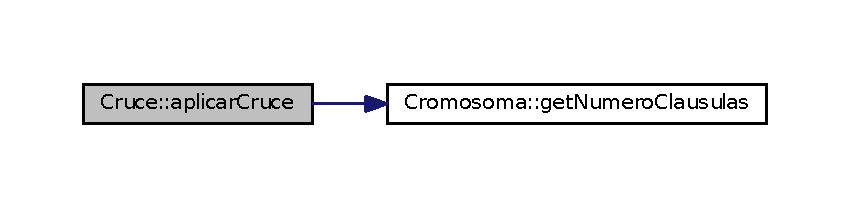
\includegraphics[width=350pt]{classCruce_a5fd9d9cbca36abf7d81f5eedc06f18e7_cgraph}
\end{center}
\end{figure}




La documentación para esta clase fue generada a partir de los siguientes ficheros\-:\begin{DoxyCompactItemize}
\item 
cruce.\-h\item 
cruce.\-cpp\end{DoxyCompactItemize}

\hypertarget{classFuncionAptitud}{\section{Referencia de la Clase Funcion\-Aptitud}
\label{classFuncionAptitud}\index{Funcion\-Aptitud@{Funcion\-Aptitud}}
}


Clase para el manejo de la función de Aptitud.  




{\ttfamily \#include $<$funcionaptitud.\-h$>$}

\subsection*{Estructuras de datos}
\begin{DoxyCompactItemize}
\item 
struct \hyperlink{structFuncionAptitud_1_1compare}{compare}
\end{DoxyCompactItemize}
\subsection*{Métodos públicos}
\begin{DoxyCompactItemize}
\item 
\hyperlink{classFuncionAptitud_a31336bdb3aa833da6c06f6b27e47522b}{Funcion\-Aptitud} (vector$<$ \hyperlink{classCromosoma}{Cromosoma} $\ast$ $>$ poblacion, \hyperlink{classTablaDeVerdad}{Tabla\-De\-Verdad} $\ast$tabla\-Verdad, bool es\-Min\-Termino)
\begin{DoxyCompactList}\small\item\em Constructor. \end{DoxyCompactList}\item 
vector$<$ \hyperlink{classCromosoma}{Cromosoma} $\ast$ $>$ \hyperlink{classFuncionAptitud_a205f0e06db47f30aa8fdce674a41b94b}{aplicar\-Aptitud} ()
\begin{DoxyCompactList}\small\item\em Función que calculara a cada cromosoma la función de aptitud y retornara la población ordena. \end{DoxyCompactList}\item 
double \hyperlink{classFuncionAptitud_a4719bc3182eeba62dd27a595f659ee8c}{obtener\-Mejor\-Aptitud} ()
\begin{DoxyCompactList}\small\item\em Función que retorna el valor de la mejor aptitud calculada. \end{DoxyCompactList}\end{DoxyCompactItemize}


\subsection{Descripción detallada}
Clase para el manejo de la función de Aptitud. 

\begin{DoxyVerb}Clase aptitud
\end{DoxyVerb}


Esta clase permitira el calculo de la función de aptitud para cada elemento e la población de Cromosomas y poder obtenerlos de manera ordenada. \begin{DoxyAuthor}{Autor}
Carlos Andres Delgado 

Edgar Andres Moncada 

Luis Felipe Vargas 
\end{DoxyAuthor}
\begin{DoxyVersion}{Versión}
1.\-0 
\end{DoxyVersion}
\begin{DoxyDate}{Fecha}
2012 
\end{DoxyDate}
\begin{DoxyCopyright}{Copyright}
G\-N\-U Public License. 
\end{DoxyCopyright}


\subsection{Documentación del constructor y destructor}
\hypertarget{classFuncionAptitud_a31336bdb3aa833da6c06f6b27e47522b}{\index{Funcion\-Aptitud@{Funcion\-Aptitud}!Funcion\-Aptitud@{Funcion\-Aptitud}}
\index{Funcion\-Aptitud@{Funcion\-Aptitud}!FuncionAptitud@{Funcion\-Aptitud}}
\subsubsection[{Funcion\-Aptitud}]{\setlength{\rightskip}{0pt plus 5cm}Funcion\-Aptitud\-::\-Funcion\-Aptitud (
\begin{DoxyParamCaption}
\item[{vector$<$ {\bf Cromosoma} $\ast$ $>$}]{poblacion, }
\item[{{\bf Tabla\-De\-Verdad} $\ast$}]{tabla\-Verdad, }
\item[{bool}]{es\-Min\-Termino}
\end{DoxyParamCaption}
)}}\label{classFuncionAptitud_a31336bdb3aa833da6c06f6b27e47522b}


Constructor. 

Constructor para la aplicación y calculo de la función de aptitud para cada \hyperlink{classCromosoma}{Cromosoma}. 
\begin{DoxyParams}{Parámetros}
{\em poblacion} & es un vector que contendrá la población de cromosomas. \\
\hline
{\em tabla\-Verdad} & es la tabla de verdad para obtener el valor de la funcion. \\
\hline
{\em es\-Min\-Termino} & variable booleana que indica si se trabaja con mini términos o maxi términos. \\
\hline
\end{DoxyParams}


\subsection{Documentación de las funciones miembro}
\hypertarget{classFuncionAptitud_a205f0e06db47f30aa8fdce674a41b94b}{\index{Funcion\-Aptitud@{Funcion\-Aptitud}!aplicar\-Aptitud@{aplicar\-Aptitud}}
\index{aplicar\-Aptitud@{aplicar\-Aptitud}!FuncionAptitud@{Funcion\-Aptitud}}
\subsubsection[{aplicar\-Aptitud}]{\setlength{\rightskip}{0pt plus 5cm}vector$<$ {\bf Cromosoma} $\ast$ $>$ Funcion\-Aptitud\-::aplicar\-Aptitud (
\begin{DoxyParamCaption}
{}
\end{DoxyParamCaption}
)}}\label{classFuncionAptitud_a205f0e06db47f30aa8fdce674a41b94b}


Función que calculara a cada cromosoma la función de aptitud y retornara la población ordena. 

\begin{DoxyReturn}{Devuelve}
un vector con los cromosomas ordenados de mejor aptitud a peor aptitud. 
\end{DoxyReturn}
por cada cromosoma

para cada valor de verdad

esta es la aptitud no la normalizacion

ordena sobre el vector de entrada

Gráfico de llamadas para esta función\-:\nopagebreak
\begin{figure}[H]
\begin{center}
\leavevmode
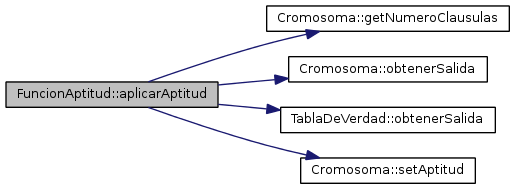
\includegraphics[width=350pt]{classFuncionAptitud_a205f0e06db47f30aa8fdce674a41b94b_cgraph}
\end{center}
\end{figure}


\hypertarget{classFuncionAptitud_a4719bc3182eeba62dd27a595f659ee8c}{\index{Funcion\-Aptitud@{Funcion\-Aptitud}!obtener\-Mejor\-Aptitud@{obtener\-Mejor\-Aptitud}}
\index{obtener\-Mejor\-Aptitud@{obtener\-Mejor\-Aptitud}!FuncionAptitud@{Funcion\-Aptitud}}
\subsubsection[{obtener\-Mejor\-Aptitud}]{\setlength{\rightskip}{0pt plus 5cm}double Funcion\-Aptitud\-::obtener\-Mejor\-Aptitud (
\begin{DoxyParamCaption}
{}
\end{DoxyParamCaption}
)}}\label{classFuncionAptitud_a4719bc3182eeba62dd27a595f659ee8c}


Función que retorna el valor de la mejor aptitud calculada. 

\begin{DoxyReturn}{Devuelve}
un double con el valor de la mejor aptitud. 
\end{DoxyReturn}


La documentación para esta clase fue generada a partir de los siguientes ficheros\-:\begin{DoxyCompactItemize}
\item 
funcionaptitud.\-h\item 
funcionaptitud.\-cpp\end{DoxyCompactItemize}

\hypertarget{classFuncionSeleccionCruce}{\section{Funcion\-Seleccion\-Cruce Class Reference}
\label{classFuncionSeleccionCruce}\index{Funcion\-Seleccion\-Cruce@{Funcion\-Seleccion\-Cruce}}
}


Clase para seleccionar el Mating pool.  




{\ttfamily \#include $<$funcion\-Seleccion\-Cruce.\-h$>$}

\subsection*{Public Member Functions}
\begin{DoxyCompactItemize}
\item 
\hyperlink{classFuncionSeleccionCruce_a22066e85dbf1ee971ff1433024ea3817}{Funcion\-Seleccion\-Cruce} (vector$<$ \hyperlink{classCromosoma}{Cromosoma} $>$ poblacion, double mejor\-Aptitud)
\begin{DoxyCompactList}\small\item\em Constructor. \end{DoxyCompactList}\item 
vector$<$ \hyperlink{classCromosoma}{Cromosoma} $>$ \hyperlink{classFuncionSeleccionCruce_a54ddbbce4b3bf60a646f28fab74b46e0}{aplicar\-Seleccion\-Cruce} ()
\begin{DoxyCompactList}\small\item\em Función que calculará los cromosomas seleccionados para relizar el cruce. \end{DoxyCompactList}\end{DoxyCompactItemize}


\subsection{Detailed Description}
Clase para seleccionar el Mating pool. 

\begin{DoxyVerb}Clase FuncionSeleccionCruce
\end{DoxyVerb}


Esta clase permitira seleccionar los cromosomas de acuerdo a la aptitud para la realización del cruce. \begin{DoxyAuthor}{Author}
Carlos Andres Delgado 

Edgar Andres Moncada 

Luis Felipe Vargas 
\end{DoxyAuthor}
\begin{DoxyVersion}{Version}
1.\-0 
\end{DoxyVersion}
\begin{DoxyDate}{Date}
2012 
\end{DoxyDate}
\begin{DoxyCopyright}{Copyright}
G\-N\-U Public License. 
\end{DoxyCopyright}


\subsection{Constructor \& Destructor Documentation}
\hypertarget{classFuncionSeleccionCruce_a22066e85dbf1ee971ff1433024ea3817}{\index{Funcion\-Seleccion\-Cruce@{Funcion\-Seleccion\-Cruce}!Funcion\-Seleccion\-Cruce@{Funcion\-Seleccion\-Cruce}}
\index{Funcion\-Seleccion\-Cruce@{Funcion\-Seleccion\-Cruce}!FuncionSeleccionCruce@{Funcion\-Seleccion\-Cruce}}
\subsubsection[{Funcion\-Seleccion\-Cruce}]{\setlength{\rightskip}{0pt plus 5cm}Funcion\-Seleccion\-Cruce\-::\-Funcion\-Seleccion\-Cruce (
\begin{DoxyParamCaption}
\item[{vector$<$ {\bf Cromosoma} $>$}]{poblacion, }
\item[{double}]{mejor\-Aptitud}
\end{DoxyParamCaption}
)}}\label{classFuncionSeleccionCruce_a22066e85dbf1ee971ff1433024ea3817}


Constructor. 

Constructor para la aplicación del Mating pool. 
\begin{DoxyParams}{Parameters}
{\em poblacion} & es un vector que contendrá la población de cromosomas. \\
\hline
{\em mejor\-Aptitud} & es el valor con la mejor aptitud, esto para calcular la normalización y que quede entre \mbox{[}0,1\mbox{]}. Se obtiene de la funcion de aptitud. \\
\hline
\end{DoxyParams}


\subsection{Member Function Documentation}
\hypertarget{classFuncionSeleccionCruce_a54ddbbce4b3bf60a646f28fab74b46e0}{\index{Funcion\-Seleccion\-Cruce@{Funcion\-Seleccion\-Cruce}!aplicar\-Seleccion\-Cruce@{aplicar\-Seleccion\-Cruce}}
\index{aplicar\-Seleccion\-Cruce@{aplicar\-Seleccion\-Cruce}!FuncionSeleccionCruce@{Funcion\-Seleccion\-Cruce}}
\subsubsection[{aplicar\-Seleccion\-Cruce}]{\setlength{\rightskip}{0pt plus 5cm}vector$<$ {\bf Cromosoma} $>$ Funcion\-Seleccion\-Cruce\-::aplicar\-Seleccion\-Cruce (
\begin{DoxyParamCaption}
{}
\end{DoxyParamCaption}
)}}\label{classFuncionSeleccionCruce_a54ddbbce4b3bf60a646f28fab74b46e0}


Función que calculará los cromosomas seleccionados para relizar el cruce. 

\begin{DoxyReturn}{Returns}
un vector con los cromosomas seleccionados. 
\end{DoxyReturn}
se calculan las puntuaciones acumuladas

constante a la mitad de la poblacion

se selecciona la posicion donde r cayo en \char`\"{}la ruleta\char`\"{}

mirando el algoritmo por internet dice que puede repetirse elementos, asi el erase no iria 

The documentation for this class was generated from the following files\-:\begin{DoxyCompactItemize}
\item 
funcion\-Seleccion\-Cruce.\-h\item 
funcion\-Seleccion\-Cruce.\-cpp\end{DoxyCompactItemize}

\hypertarget{classMutacion}{\section{Referencia de la Clase Mutacion}
\label{classMutacion}\index{Mutacion@{Mutacion}}
}


Clase para implementar mutación.  




{\ttfamily \#include $<$mutacion.\-h$>$}

\subsection*{Métodos públicos}
\begin{DoxyCompactItemize}
\item 
\hyperlink{classMutacion_afee3c90f0afc795c89fa0590bef2b667}{Mutacion} (vector$<$ \hyperlink{classCromosoma}{Cromosoma} $>$ hijos)
\begin{DoxyCompactList}\small\item\em Constructor. \end{DoxyCompactList}\item 
vector$<$ \hyperlink{classCromosoma}{Cromosoma} $>$ \hyperlink{classMutacion_a6ef8eb8c3818175895cf7ff56cdfedf0}{aplicar\-Mutacion} ()
\end{DoxyCompactItemize}


\subsection{Descripción detallada}
Clase para implementar mutación. 

\begin{DoxyVerb}Clase Mutacion
\end{DoxyVerb}


Para mutar se selecciona el 2 \% de los individuos, en éstos se selecciona aleatoriamente una claúsula, con probabilidad del 50 \% se realiza alguna de estas dos acciones. $\ast$ Borrar claúsula Borra una clausula, si es la única de la función, la salida de la misma es siempre 0.\-Cambiar el valor de una variable Se selecciona una posición de la claúsula y se cambia el valor que tiene asignado por su negación. \begin{DoxyAuthor}{Autor}
Carlos Andres Delgado 

Edgar Andres Moncada 

Luis Felipe Vargas 
\end{DoxyAuthor}
\begin{DoxyVersion}{Versión}
1.\-0 
\end{DoxyVersion}
\begin{DoxyDate}{Fecha}
2012 
\end{DoxyDate}
\begin{DoxyCopyright}{Copyright}
G\-N\-U Public License. 
\end{DoxyCopyright}


\subsection{Documentación del constructor y destructor}
\hypertarget{classMutacion_afee3c90f0afc795c89fa0590bef2b667}{\index{Mutacion@{Mutacion}!Mutacion@{Mutacion}}
\index{Mutacion@{Mutacion}!Mutacion@{Mutacion}}
\subsubsection[{Mutacion}]{\setlength{\rightskip}{0pt plus 5cm}Mutacion\-::\-Mutacion (
\begin{DoxyParamCaption}
\item[{vector$<$ {\bf Cromosoma} $>$}]{hijos}
\end{DoxyParamCaption}
)}}\label{classMutacion_afee3c90f0afc795c89fa0590bef2b667}


Constructor. 

Constructor para la aplicación de la mutación de los hijos generados de la población de Cromosomas 
\begin{DoxyParams}{Parámetros}
{\em poblacion} & es un vector que contiene los hijos generados en el \hyperlink{classCruce}{Cruce}. \\
\hline
\end{DoxyParams}


\subsection{Documentación de las funciones miembro}
\hypertarget{classMutacion_a6ef8eb8c3818175895cf7ff56cdfedf0}{\index{Mutacion@{Mutacion}!aplicar\-Mutacion@{aplicar\-Mutacion}}
\index{aplicar\-Mutacion@{aplicar\-Mutacion}!Mutacion@{Mutacion}}
\subsubsection[{aplicar\-Mutacion}]{\setlength{\rightskip}{0pt plus 5cm}vector$<$ {\bf Cromosoma} $>$ Mutacion\-::aplicar\-Mutacion (
\begin{DoxyParamCaption}
{}
\end{DoxyParamCaption}
)}}\label{classMutacion_a6ef8eb8c3818175895cf7ff56cdfedf0}
Funcion que mutara a los Cromosomas hijos el 2\% de la población.

\begin{DoxyVerb}  \return un vector con los cromosomas hijos ya mutados.\end{DoxyVerb}
 

La documentación para esta clase fue generada a partir de los siguientes ficheros\-:\begin{DoxyCompactItemize}
\item 
mutacion.\-h\item 
mutacion.\-cpp\end{DoxyCompactItemize}

\hypertarget{classSeleccion}{\section{Referencia de la Clase Seleccion}
\label{classSeleccion}\index{Seleccion@{Seleccion}}
}


Clase para el manejo de la función de Aptitud.  




{\ttfamily \#include $<$seleccion.\-h$>$}

\subsection*{Métodos públicos}
\begin{DoxyCompactItemize}
\item 
\hyperlink{classSeleccion_a98fa8d406a3f543405dab4f25efde0a0}{Seleccion} (vector$<$ \hyperlink{classCromosoma}{Cromosoma} $>$ poblacion, vector$<$ \hyperlink{classCromosoma}{Cromosoma} $>$ hijos)
\begin{DoxyCompactList}\small\item\em Constructor. \end{DoxyCompactList}\item 
vector$<$ \hyperlink{classCromosoma}{Cromosoma} $>$ \hyperlink{classSeleccion_ae8ac58d7995c5807522fa3eba7a17ebb}{aplicar\-Seleccion} ()
\end{DoxyCompactItemize}


\subsection{Descripción detallada}
Clase para el manejo de la función de Aptitud. 

\begin{DoxyVerb}Clase Seleccion
\end{DoxyVerb}


Esta clase permitira el calculo de la función de aptitud para cada elemento e la población de Cromosomas y poder obtenerlos de manera ordenada. \begin{DoxyAuthor}{Autor}
Carlos Andres Delgado 

Edgar Andres Moncada 

Luis Felipe Vargas 
\end{DoxyAuthor}
\begin{DoxyVersion}{Versión}
1.\-0 
\end{DoxyVersion}
\begin{DoxyDate}{Fecha}
2012 
\end{DoxyDate}
\begin{DoxyCopyright}{Copyright}
G\-N\-U Public License. 
\end{DoxyCopyright}


\subsection{Documentación del constructor y destructor}
\hypertarget{classSeleccion_a98fa8d406a3f543405dab4f25efde0a0}{\index{Seleccion@{Seleccion}!Seleccion@{Seleccion}}
\index{Seleccion@{Seleccion}!Seleccion@{Seleccion}}
\subsubsection[{Seleccion}]{\setlength{\rightskip}{0pt plus 5cm}Seleccion\-::\-Seleccion (
\begin{DoxyParamCaption}
\item[{vector$<$ {\bf Cromosoma} $>$}]{poblacion, }
\item[{vector$<$ {\bf Cromosoma} $>$}]{hijos}
\end{DoxyParamCaption}
)}}\label{classSeleccion_a98fa8d406a3f543405dab4f25efde0a0}


Constructor. 

Constructor para la aplicación de la seleccion de cromosomas 
\begin{DoxyParams}{Parámetros}
{\em poblacion} & es un vector que contendrá la población de cromosomas viejas. \\
\hline
{\em hijos} & es un vector que contendrá la población de cromosomas que se ha cruzado y aplicado posibles mutaciones. \\
\hline
\end{DoxyParams}


\subsection{Documentación de las funciones miembro}
\hypertarget{classSeleccion_ae8ac58d7995c5807522fa3eba7a17ebb}{\index{Seleccion@{Seleccion}!aplicar\-Seleccion@{aplicar\-Seleccion}}
\index{aplicar\-Seleccion@{aplicar\-Seleccion}!Seleccion@{Seleccion}}
\subsubsection[{aplicar\-Seleccion}]{\setlength{\rightskip}{0pt plus 5cm}vector$<$ {\bf Cromosoma} $>$ Seleccion\-::aplicar\-Seleccion (
\begin{DoxyParamCaption}
{}
\end{DoxyParamCaption}
)}}\label{classSeleccion_ae8ac58d7995c5807522fa3eba7a17ebb}
Función seleccionara, por medio del metodo de seleccion por ruleta, entre la población vieja y los hijos mutados para que pasen a la siguiente generación.

\begin{DoxyVerb}  \return un vector con los cromosomas seleccionados del mismo tamaño de la población inicial.\end{DoxyVerb}
 

La documentación para esta clase fue generada a partir de los siguientes ficheros\-:\begin{DoxyCompactItemize}
\item 
seleccion.\-h\item 
seleccion.\-cpp\end{DoxyCompactItemize}

\hypertarget{classTablaDeVerdad}{\section{Referencia de la Clase Tabla\-De\-Verdad}
\label{classTablaDeVerdad}\index{Tabla\-De\-Verdad@{Tabla\-De\-Verdad}}
}


Clase \hyperlink{classTablaDeVerdad}{Tabla\-De\-Verdad}.  




{\ttfamily \#include $<$Tabla\-De\-Verdad.\-h$>$}

\subsection*{Métodos públicos}
\begin{DoxyCompactItemize}
\item 
\hyperlink{classTablaDeVerdad_a69d50b7f18461c771ceb15b14a660122}{Tabla\-De\-Verdad} ()
\begin{DoxyCompactList}\small\item\em Constructor. \end{DoxyCompactList}\item 
\hyperlink{classTablaDeVerdad_ac41dd0d65d191b0a34b369b8a4d2439d}{$\sim$\-Tabla\-De\-Verdad} ()
\begin{DoxyCompactList}\small\item\em Destructor. \end{DoxyCompactList}\item 
bool \hyperlink{classTablaDeVerdad_a3e53eabc4e37d9514141f4afacc1e915}{obtener\-Salida} (int posicion\-Decimal)
\begin{DoxyCompactList}\small\item\em obtener\-Salida \end{DoxyCompactList}\item 
void \hyperlink{classTablaDeVerdad_add681181eba54bcb2f1153c6f886a793}{escribir\-Tabla\-De\-Verdad} (bool valor)
\begin{DoxyCompactList}\small\item\em escribir\-Tabla\-De\-Verdad \end{DoxyCompactList}\end{DoxyCompactItemize}


\subsection{Descripción detallada}
Clase \hyperlink{classTablaDeVerdad}{Tabla\-De\-Verdad}. 

\begin{DoxyVerb}Clase cromosoma
\end{DoxyVerb}


Define la tabla de verdad de la entrada \begin{DoxyAuthor}{Autor}
Carlos Andres Delgado 

Edgar Andres Moncada 

Luis Felipe Vargas 
\end{DoxyAuthor}
\begin{DoxyVersion}{Versión}
1.\-0 
\end{DoxyVersion}
\begin{DoxyDate}{Fecha}
2012 
\end{DoxyDate}
\begin{DoxyCopyright}{Copyright}
G\-N\-U Public License. 
\end{DoxyCopyright}


\subsection{Documentación del constructor y destructor}
\hypertarget{classTablaDeVerdad_a69d50b7f18461c771ceb15b14a660122}{\index{Tabla\-De\-Verdad@{Tabla\-De\-Verdad}!Tabla\-De\-Verdad@{Tabla\-De\-Verdad}}
\index{Tabla\-De\-Verdad@{Tabla\-De\-Verdad}!TablaDeVerdad@{Tabla\-De\-Verdad}}
\subsubsection[{Tabla\-De\-Verdad}]{\setlength{\rightskip}{0pt plus 5cm}Tabla\-De\-Verdad\-::\-Tabla\-De\-Verdad (
\begin{DoxyParamCaption}
{}
\end{DoxyParamCaption}
)}}\label{classTablaDeVerdad_a69d50b7f18461c771ceb15b14a660122}


Constructor. 

Constructor de la clase \hyperlink{classCromosoma}{Cromosoma} \hypertarget{classTablaDeVerdad_ac41dd0d65d191b0a34b369b8a4d2439d}{\index{Tabla\-De\-Verdad@{Tabla\-De\-Verdad}!$\sim$\-Tabla\-De\-Verdad@{$\sim$\-Tabla\-De\-Verdad}}
\index{$\sim$\-Tabla\-De\-Verdad@{$\sim$\-Tabla\-De\-Verdad}!TablaDeVerdad@{Tabla\-De\-Verdad}}
\subsubsection[{$\sim$\-Tabla\-De\-Verdad}]{\setlength{\rightskip}{0pt plus 5cm}Tabla\-De\-Verdad\-::$\sim$\-Tabla\-De\-Verdad (
\begin{DoxyParamCaption}
{}
\end{DoxyParamCaption}
)}}\label{classTablaDeVerdad_ac41dd0d65d191b0a34b369b8a4d2439d}


Destructor. 

Destructor de la clase \hyperlink{classCromosoma}{Cromosoma} 

\subsection{Documentación de las funciones miembro}
\hypertarget{classTablaDeVerdad_add681181eba54bcb2f1153c6f886a793}{\index{Tabla\-De\-Verdad@{Tabla\-De\-Verdad}!escribir\-Tabla\-De\-Verdad@{escribir\-Tabla\-De\-Verdad}}
\index{escribir\-Tabla\-De\-Verdad@{escribir\-Tabla\-De\-Verdad}!TablaDeVerdad@{Tabla\-De\-Verdad}}
\subsubsection[{escribir\-Tabla\-De\-Verdad}]{\setlength{\rightskip}{0pt plus 5cm}void Tabla\-De\-Verdad\-::escribir\-Tabla\-De\-Verdad (
\begin{DoxyParamCaption}
\item[{bool}]{valor}
\end{DoxyParamCaption}
)}}\label{classTablaDeVerdad_add681181eba54bcb2f1153c6f886a793}


escribir\-Tabla\-De\-Verdad 

Escribe una salida para la entrada en orden 
\begin{DoxyParams}{Parámetros}
{\em valor} & booleano que indica la entrada \\
\hline
\end{DoxyParams}
\hypertarget{classTablaDeVerdad_a3e53eabc4e37d9514141f4afacc1e915}{\index{Tabla\-De\-Verdad@{Tabla\-De\-Verdad}!obtener\-Salida@{obtener\-Salida}}
\index{obtener\-Salida@{obtener\-Salida}!TablaDeVerdad@{Tabla\-De\-Verdad}}
\subsubsection[{obtener\-Salida}]{\setlength{\rightskip}{0pt plus 5cm}bool Tabla\-De\-Verdad\-::obtener\-Salida (
\begin{DoxyParamCaption}
\item[{int}]{posicion\-Decimal}
\end{DoxyParamCaption}
)}}\label{classTablaDeVerdad_a3e53eabc4e37d9514141f4afacc1e915}


obtener\-Salida 

Obtiene una salida ante una entrada decimal de la entrada 
\begin{DoxyParams}{Parámetros}
{\em posicion\-Decimal} & es un número entero que representa la posición que se desea conocer \\
\hline
\end{DoxyParams}
\begin{DoxyReturn}{Devuelve}
booleano que representa el valor que toma la tabla de verdad ante la entrada especificada 
\end{DoxyReturn}


Gráfico de llamadas a esta función\-:
\nopagebreak
\begin{figure}[H]
\begin{center}
\leavevmode
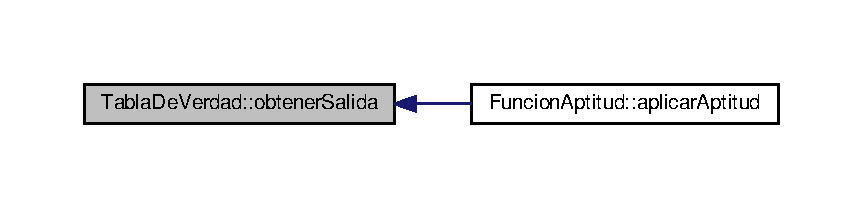
\includegraphics[width=350pt]{classTablaDeVerdad_a3e53eabc4e37d9514141f4afacc1e915_icgraph}
\end{center}
\end{figure}




La documentación para esta clase fue generada a partir de los siguientes ficheros\-:\begin{DoxyCompactItemize}
\item 
Tabla\-De\-Verdad.\-h\item 
Tabla\-De\-Verdad.\-cpp\end{DoxyCompactItemize}

\printindex
\end{document}
